\chapter{语法检查}

\begin{introduction}
    \item 建议认真阅读 Yx\cite{Yx} 的代码和里面的 Tutorial.md。
    \item 一些建议:多和同学、助教交流。
\end{introduction}

% \noindent
% (先写一点备注) \\
% 1. 强烈建议认真阅读Yx的代码和Tutorial.md。 \\
% Yx是一个比Mx*更加简单的语法,阅读Yx的实现对于代码的完成非常有帮助。\\
% Yx的github地址:https://github.com/ZYHowell/Yx \\
% 2. 一些建议:多和同学、助教交流;没有头绪时多看看Yx和学长学姐的代码,有助于理解并提高效率;
% 切忌抄袭。\\

\section{语法检查摘要}
语法检查阶段需要完成词法分析、语法分析、语义分析。在本作业中,
词法分析和语法分析可以使用现有的分析库将源代码转换为语法树。
随后,你可以将具象语法树转换为抽象语法树 (Abstract Syntax Tree, AST)
从而更好地表达代码的结构。本阶段的最后一步需要你在树(语法树和抽象语法树均可)上进行语法检查
(例如:简单的类型检查、if/while/for 等语句的表达式合法性等),确保代码符合规则。

接下来,我们将首先讲解对于 semantic 阶段工作的整体理解,再对具体的实现步骤逐步解析。

\begin{remark}
    \textbf{本章节的示例为语言为 Java,语法分析器为 ANTLR。}
\end{remark}

\section{总览}
语法检查阶段的难点都与抽象语法树 (Abstract Syntax Tree, AST)
有关,分别是如何构建 AST 以及如何在 AST 上遍历进行语法检查。
两个步骤的难点主要在工程实现。ANTLR 能够将我们编写的语法规则(g4 文件)生成对应的
parser 和 lexer,并构建一棵语法树。ANTLR 为这棵语法树提供了 listener 和 visitor
的接口,便于我们提取其中的信息,我们希望能够自定义树的每个结点,并储存需要的信息。
因此,我们将继承 ANTLR 生成的 listener 或 visitor,通过遍历具象语法树构建一棵抽象语法树。
最后,在抽象语法树上进行遍历,对源代码的语法进行检查。

分步骤来看,这个阶段你需要完成的任务有:
\begin{enumerate}
    \item 为语言编写文法分析文件(g4 文件);
    \item 继承 ANTLR 生成的 visitor 或 listener 实现对 ANTLR 的语法树遍历,并同时构建抽象语法树(可选);
    \item 遍历语法树或抽象语法树对源代码进行语法检查。
\end{enumerate}

% 一份Mx*代码将被转换成一棵AST,这棵树从RootNode开始,随着树的层数的加深,
% 每层的结点所表示的单位逐渐变小。下面是基于Mx*的一个AST层级的简单示意:
% \begin{lstlisting}
% RootNode 
% - VariableDef
% - ClassDefinition
%     - VariableDefinition
%     - FuncDefinition
% - FunctionDefinition - Statements - Expressions 
% \end{lstlisting}

% Mx*语言下,对这个结构进行一点简单的注解:\\
% 1. RootNode从全局作用域开始。Mx*的全局作用域中只存在全局变量、类定义、全局函数三种类型。\\
% 2. 类定义中,只存在变量和函数。 \\
% 3. 一个函数包含多个statement(语句)。在AST中,一个函数中的每个statement都是这个函数节点的子节点。
% statement有许多种类型,比如if语句、循环语句(for、while)等等。\\
% 4. expression(表达式)有许多种类型,比如基本表达式(primary)、常量表达式(constant)、赋值表达式(assignment)等等。 \\
% 5. 关于Mx*所使用的statement和expression,Mx*文档中均有明确的规定,概念模糊的同学可以先仔细阅读。 \\

% 如果你对以上结构感到费解,可以仔细阅读Yx库中的g4文件(Yx/src/parser/Yx.g4)辅助理解,或者继续阅读下一部分中对于如何构建AST的详细介绍,
% 准确地理解AST的结构将会大大提高效率。\\

% \section{实现方法概述}
% 在这一部分,我们将逐任务剖析如何完成语法检查阶段。

\section{语法分析}
\subsection{语法描述文件}
我们采用 ANTLR 构建语法树,我们需要先写一个 Mx*.g4 文件,用来描述 Mx* 的语法。在这里我们以 Yx-Compiler\cite{Yx}
为例子讲述如何撰写一个 ANTLR 下的语法描述文件。

首先我们需要定义词法,以下的代码将 \texttt{int} 字符串识别为 \texttt{Int},
将整数(以 1-9 开头且以 0-9 为后续字符的字符串、字符 0)识别为 \texttt{DecimalInteger}。
(思考:这里如果要支持小数该怎么写呢?)词法规则是有顺序的,在下面的例子中,\texttt{int}
既可以是 \texttt{Int},也可以是 \texttt{Identifier},但我们只希望它被识别为 \texttt{Int},
所以我们将 \texttt{Int} 写在前面。
\begin{lstlisting}
Int : 'int';
DecimalInteger
    : [1-9] [0-9]*
    | '0'
    ;
Identifier : [a-zA-Z] [a-zA-Z_0-9]*;
\end{lstlisting}



撰写完成词法规则之后,需要撰写对应的语法规则。
在介绍这部分之前,我们先对语句类型进行简单的划分。
一个函数包含多个 statement (语句),statement 有许多种类型,比如 if 语句、循环语句 (for、while) 等等。
注意,书写这部分之前,需要先对抽象语法树上可能存在的节点有个大致的规划。一般地,我们会设计 \texttt{Statement}
抽象类和 \texttt{Expression} 抽象类。
所有具体的语句都继承 \texttt{Statement},各种具体的表达式都继承 \texttt{Expression}。
而针对具体的语句,需要根据语法定义要求规划节点类型。
例如,对if语句 (\texttt{IfStmt}) 节点,需要包括一个表达式节点 (\texttt{ExpressionNode})
表达条件,两个语句 (statements) 分别代表条件为真 (True Statement) 或假 (False Statement) 的语句。

以 Yx 的 \texttt{Statement} 部分为例:
\begin{lstlisting}
statement
    : suite                                                 #block
    | varDef                                                #vardefStmt
    | If '(' expression ')' trueStmt=statement 
        (Else falseStmt=statement)?                         #ifStmt
    | Return expression? ';'                                #returnStmt
    | expression ';'                                        #pureExprStmt
    | ';'                                                   #emptyStmt
    ;
\end{lstlisting}
在这部分代码中,定义了 \texttt{statement}
包括 \texttt{ifStmt}、\texttt{returnStmt} 等几种\texttt{Statement},
而 \texttt{ifStmt} 中表达式节点将会被解析为 \texttt{expression}
(在 ANTLR 的 Visitor 中为 \texttt{visitifStmt} 函数的 \texttt{ctx.expression()}),另外两个
statement 将会被分别解析为 \texttt{trueStmt} 和\texttt{falseStmt}。


当你完成词法和语法对应规则的书写之后,语法描述文件的实现完成。以下是一些小贴士:
\begin{enumerate}
    \item 对于 Mx*,如果觉得 Lexer 和 Parser 置于同一文件中过于复杂,可以考虑分为两个文件(Mx*Lexer.g4, Mx*Parser.g4)来书写。
    \item 如果你使用 IDEA,可以基于你写的 g4 文件,输入一段 Mx* 代码,可视化地生成解析树。效果大致如下,具体方法可自行查阅。
    \item antlr4 的其他详细内容,请参照《antlr4 权威指南》。
\end{enumerate}

\begin{figure}[htbp]
    \centering
    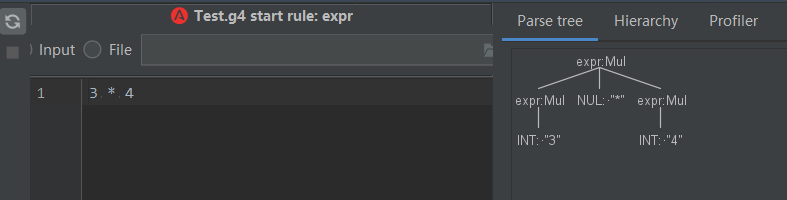
\includegraphics[width=0.7\textwidth]{image/g4.png}
    \caption{样例}
\end{figure}

\section{抽象语法树}

将撰写的 g4 文件传递给 ANTLR 后,ANTLR 会生成以下文件(以 Yx 为例):
\begin{enumerate}
    \item YxLexer.java - 词法分析器。
    \item YxParser.java - 语法分析器,用于生成语法树。
    \item YxBaseListener.java - Listener 类,用于遍历语法树。
    \item YxBaseVisitor.java - Visitor 类,用于遍历语法树。
    \item YxListener.java - Listener 接口。
    \item YxVisitor.java - Visitor 接口。
\end{enumerate}
Listener 和 Visitor 是 antlr4 提供的两种遍历方法。两者的具体意义《antlr4 权威指南》(49 页起)有详细说明。
这些 Listener 和 Visitor 可以被用于遍历语法树。在此之前,我们先调用如下代码让 ANTLR 构建语法树,\texttt{parseTreeRoot}
即为语法树的根节点。
\begin{lstlisting}[language=Java]
YxLexer lexer = new YxLexer(CharStreams.fromStream(input));
lexer.removeErrorListeners();
lexer.addErrorListener(new YxErrorListener());
YxParser parser = new YxParser(new CommonTokenStream(lexer));
parser.removeErrorListeners();
parser.addErrorListener(new YxErrorListener());
ParseTree parseTreeRoot = parser.program();
\end{lstlisting}

\begin{remark}
    ANTLR 在 lexer 和 parser 的过程中,能够发现词法、语法错误,而具体的异常类可以自定义。\textbf{并不是所有 ANTLR 抛出的错误都是需要处理的错误。}具体请参考 Yx 对于 \texttt{YxErrorListener} 类的处理。
\end{remark}

\subsection{AST 节点}
现在,我们可以通过变量 \texttt{parseTreeRoot} 得到语法树的根节点,并建一棵 AST。
那么首先,我们需要为每一个节点定义一个类,来保存各自需要的信息,从而构成一棵树。
这里的树形结构和 g4 的语法结构本质上是一致的。
以下是 Yx 给出的 \texttt{ifStmtNode} 类的定义作为例子:
\begin{lstlisting}[language=Java]
abstract public class ASTNode {
    public position pos; // 用于存储节点所指代的对源代码范围
    public ASTNode(position pos) {
        this.pos = pos;
    }
    // 每个 ASTNode 都包括一个 accept 方法,可以用来遍历 AST
    abstract public void accept(ASTVisitor visitor);
}
// Statement 的抽象类,所有的 Statement 继承自这个节点。
// 同时这个节点也是 ASTNode 的派生类。
public abstract class StmtNode extends ASTNode {
    public StmtNode(position pos) {
        super(pos);
    }
}

public class ifStmtNode extends StmtNode {
    ExprNode condition; // 用于存储 Expression(条件)
    StmtNode thenStmt, elseStmt; // 分别用于存储上文的 trueStmt 和 falseStmt
    public ifStmtNode(ExprNode condition, StmtNode thenStmt, StmtNode elseStmt, position pos) {
        super(pos);
        this.condition = condition;
        this.thenStmt = thenStmt;
        this.elseStmt = elseStmt;
    }
    
    // 继承 ASTNode 的 accept 方法,将会跳转到对应的 ASTVisitor 进行节点访问。
    @Override
    public void accept(ASTVisitor visitor) {
        visitor.visit(this);
    }
}
\end{lstlisting}

需要注意的是,在定义 AST 节点的过程中,对于表达式节点 (\texttt{ExprNode}),我们还需要关注它的类型。在
Mx* 语言中,允许出现的类型除了 Mx* 文档提到的 \texttt{int}, \texttt{bool} 等基础类型外,
还会出现 Mx* 代码中自定义的类,所以我们需要建立一个内部的类型系统来管理各种类型。
表现在具体的代码中,即 \texttt{ExprNode} 类中会含有一个 \texttt{Type}
型的成员变量,用来表示这个表达式对应的类型。(如下所示)
\begin{lstlisting}[language=Java]
public abstract class ExprNode extends ASTNode {
    Type type;
    public ExprNode(position pos) {
        super(pos);
    }
}
\end{lstlisting}
对于 \texttt{Type} 类,这是需要自主实现的一个类,用来根据具体的需要处理类型相关的问题
(比如如何表示自定义类、如何处理数组问题等等),\texttt{Type} 类的实现可以参考 Yx 以及他人的代码。


\subsection{构建抽象语法树 (Abstract Syntax Tree, AST)}
ANTLR 生成的文件中,\texttt{BaseVisitor} 提供了可以显式访问 parse tree 子结点的接口,所以
\texttt{ASTBuilder} 类将继承 \texttt{Mx*BaseVisitor} 类,然后访问 parse tree 的各个节点,
将需要的信息依次读入自定义的各种 \texttt{ASTNode} 类中,构建自己的 AST 树。构建 AST 的过程是一个递归的过程。

在这里,我们仍然以 if 语句为例子,在语法描述文件中,我们定义 if 语句的方式是 \texttt{If '(' expression ')' trueStmt=statement (Else falseStmt=statement)?}。
其中包括了 \texttt{expression}、\texttt{trueStmt}、\texttt{falseStmt}。
在这里,需要对每个语句中的部分构建出对应的子树并连接在一个if节点。
\begin{lstlisting}[language=Java]
@Override public ASTNode visitIfStmt(YxParser.IfStmtContext ctx) {
    // 访问并构建 trueStmt 对应的子树
    StmtNode thenStmt = (StmtNode)visit(ctx.trueStmt), elseStmt = null;
    // 访问并构建 expression 对应的子树
    ExprNode condition = (ExprNode)visit(ctx.expression());
    // 如果存在 else,那么构建对应 falseStmt 对应的子树
    if (ctx.falseStmt != null) elseStmt = (StmtNode)visit(ctx.falseStmt);
    // 将构建得到的多个子树根节点串接起来,并返回该 if 语句的根节点
    // 每个 visit 函数都会返回以当前为根的子树根节点,由此实现递归的树构建。
    return new ifStmtNode(condition, thenStmt, elseStmt, new position(ctx));
}
\end{lstlisting}


\section{语义检查}
进行到这一步,我们已经建好了AST,接下来我们将进行语义检查。

\subsection{符号}
在一段代码中,我们为了方便阅读,为每个变量、类、函数等都赋予了一个名字(我们又称为标识符)。
这些标识符正是编程中的符号的一种具体实例,符号是一种原始数据类型,且具有人类可阅读的形式 (human-readable form)。
每一个符号并不总是全局有效的。比如函数内声明的变量并不能被另外一个函数直接使用。
因此,每一个符号在源代码中拥有一段其可见和可访问的区域。对此,作用域的概念被提出用于规定代码中一个特定符号的有效范围。

% 符号(symbol): 在Mx*中,符号主要指程序中出现的变量、函数、类等。

% 作用域(scope):指程序中的某个特定位置或区域中,变量、函数、类等符号的可见性和可访问性范围,即规定了在程序中使用和访问符号的有效范围。
% 具体的说明见Mx*文档。

\subsection{作用域构建}
实现语义检查的过程中,我们需要关注对作用域 (scope) 的处理,确保符号在程序中的正确使用。
根据代码的定义,在一段代码中创建的新作用域默认可以访问更高一层次作用域内的符号。
因此,可以采用树的结构来维护符号的有效性信息,根据作用域的关系建树。
% 在Yx的示例代码中,关于Scope采用了一个类似树的结构来维护,根据作用域的关系建树。

以下以 Yx 代码中 \texttt{Scope} 类为例。首先,定义一个 \texttt{Scope} 类,用以储存每个作用域内需要的信息。
\begin{lstlisting}[language=Java]
public class Scope {
    // 用于存储符号和其对应类型信息,编译检查类型错误
    private HashMap<String, Type> members;
    public HashMap<String, register> entities = new HashMap<>();
    private Scope parentScope; // 保存外层作用域,用于回溯

    public Scope(Scope parentScope) {
        members = new HashMap<>();
        this.parentScope = parentScope;
    }
}
\end{lstlisting}

其次,以全局作用域作为根节点。在 AST 遍历器上维护一个 \texttt{currentScope}
表示当前作用域,如果产生了一个新的作用域(比如在 \texttt{IfStmtNode} 中,一个 if-else
语句会产生两个内层的作用域),则新建一个 \texttt{Scope} 类变量作为新的 \texttt{currentScope},完成
该内层作用域内的工作后,再将 \texttt{currentScope} 退回先前的作用域,通过成员变量
\texttt{parentScope} 记录作用域之间的关系并实现回溯。
这样,每当我们需要为一个被调用的变量寻找它的定义,我们可以通过 \texttt{parentScope}
从当前作用域不断向前回溯,直到找到这个变量对应的定义。举例如下:
\begin{lstlisting}[language=Java]
// 访问 AST 上的 blockStmt 节点
public void visit(blockStmtNode it) {
    if (!it.stmts.isEmpty()) {
        currentScope = new Scope(currentScope);
        // 递归访问子树,构建 Scope 关系
        for (StmtNode stmt : it.stmts) stmt.accept(this);
        currentScope = currentScope.parentScope();
    }
}
\end{lstlisting}

\subsection{符号收集}
在 Mx* 中,全局作用域内的函数和类是支持前向引用(在函数、类定义之前进行调用)的,所以需要先对全局的符号进行收集(这个过程称为 symbol collection),
并把收集的符号存储在全局作用域 (global scope) 内。

这里注意,Mx* 中有一些无需定义的基本类型、内建方法等,在初始化全局作用域时应该先行保存。更多细节可以阅读 Yx 的 Tutorial.md 中的讲解和 Yx 代码,辅助理解。

\subsection{语义检查}
在完成作用域的构建后,我们开始进行语义检查。
在这一部分,我们需要遍历 AST 所有的节点,并对每个节点可能出现的错误进行判断。
这一步在 Mx* 中需要在作用域构建之后完成以支持前向引用。

以下列举一些语义检查过程中需要进行的工作和可能遇到的错误。

\begin{enumerate}
    \item 类型检查:主要检查类型匹配问题,遍历过程中需要进行一定的类型推断。
    \item 类型推断: 遍历节点过程中,需要通过上下文信息来确定某个表达式的类型。比如 \texttt{a=b+c}
      中,\texttt{b} 和 \texttt{c} 都是 \texttt{int} 型,则可以推断二元表达式 \texttt{b+c} 也应为 \texttt{int} 型。
    \item 类型匹配: 可能的问题有函数调用的参数是否匹配、操作符对应的类型是否匹配、函数返回值的类型是否匹配、右值不能被赋值等等。
    \item 作用域: 符号的使用是否正确,有无重名、未定义符号等问题。
    \item 控制流: \texttt{break} 和 \texttt{continue} 的使用。
\end{enumerate}


Mx* 涉及的语义错误在 Mx* 文档中有详细的描述,这部分的代码相当琐碎,书写和 debug 过程中请保持耐心和细心。
具体代码可以参考 Yx 和他人的代码。

